% Options for packages loaded elsewhere
\PassOptionsToPackage{unicode}{hyperref}
\PassOptionsToPackage{hyphens}{url}
\documentclass[
]{ltjsarticle}
\usepackage{xcolor}
\usepackage{amsmath,amssymb}
\setcounter{secnumdepth}{-\maxdimen} % remove section numbering
\usepackage{iftex}
\ifPDFTeX
  \usepackage[T1]{fontenc}
  \usepackage[utf8]{inputenc}
  \usepackage{textcomp} % provide euro and other symbols
\else % if luatex or xetex
  \usepackage{unicode-math} % this also loads fontspec
  \defaultfontfeatures{Scale=MatchLowercase}
  \defaultfontfeatures[\rmfamily]{Ligatures=TeX,Scale=1}
\fi
\usepackage{lmodern}
\ifPDFTeX\else
  % xetex/luatex font selection
\fi
% Use upquote if available, for straight quotes in verbatim environments
\IfFileExists{upquote.sty}{\usepackage{upquote}}{}
\IfFileExists{microtype.sty}{% use microtype if available
  \usepackage[]{microtype}
  \UseMicrotypeSet[protrusion]{basicmath} % disable protrusion for tt fonts
}{}
\makeatletter
\@ifundefined{KOMAClassName}{% if non-KOMA class
  \IfFileExists{parskip.sty}{%
    \usepackage{parskip}
  }{% else
    \setlength{\parindent}{0pt}
    \setlength{\parskip}{6pt plus 2pt minus 1pt}}
}{% if KOMA class
  \KOMAoptions{parskip=half}}
\makeatother
\usepackage{graphicx}
\makeatletter
\newsavebox\pandoc@box
\newcommand*\pandocbounded[1]{% scales image to fit in text height/width
  \sbox\pandoc@box{#1}%
  \Gscale@div\@tempa{\textheight}{\dimexpr\ht\pandoc@box+\dp\pandoc@box\relax}%
  \Gscale@div\@tempb{\linewidth}{\wd\pandoc@box}%
  \ifdim\@tempb\p@<\@tempa\p@\let\@tempa\@tempb\fi% select the smaller of both
  \ifdim\@tempa\p@<\p@\scalebox{\@tempa}{\usebox\pandoc@box}%
  \else\usebox{\pandoc@box}%
  \fi%
}
% Set default figure placement to htbp
\def\fps@figure{htbp}
\makeatother
\setlength{\emergencystretch}{3em} % prevent overfull lines
\providecommand{\tightlist}{%
  \setlength{\itemsep}{0pt}\setlength{\parskip}{0pt}}
\usepackage{bookmark}
\IfFileExists{xurl.sty}{\usepackage{xurl}}{} % add URL line breaks if available
\urlstyle{same}
\hypersetup{
  hidelinks,
  pdfcreator={LaTeX via pandoc}}

\author{}
\date{}

\begin{document}

\section{論文1：波長空間と周波数空間の双対幾何}\label{ux8ad6ux65871ux6ce2ux9577ux7a7aux9593ux3068ux5468ux6ce2ux6570ux7a7aux9593ux306eux53ccux5bfeux5e7eux4f55}

\subsection{逆数条件・対数表現・不確定性付き数え上げに関する幾何学的・位相的観察モデル}\label{ux9006ux6570ux6761ux4ef6ux5bfeux6570ux8868ux73feux4e0dux78baux5b9aux6027ux4ed8ux304dux6570ux3048ux4e0aux3052ux306bux95a2ux3059ux308bux5e7eux4f55ux5b66ux7684ux4f4dux76f8ux7684ux89b3ux5bdfux30e2ux30c7ux30eb}

\textbf{著者}: 木原 範昭 (Noriaki Kihara)\\
\textbf{所属}: WF System Co., Ltd.\\
\textbf{ORCID}: 0009-0004-6753-4020\\
\textbf{版}: v0.3\\
\textbf{日付}: 2026 年 6 月\\
\textbf{DOI（本版）}: 10.5281/zenodo.20588037\\
\textbf{Concept DOI}: 10.5281/zenodo.20588036\\
\textbf{ライセンス}: CC BY 4.0

\begin{center}\rule{0.5\linewidth}{0.5pt}\end{center}

\subsection{要旨}\label{ux8981ux65e8}

本稿では、波長成分 \(\lambda_n\) と周波数成分 \(\nu_n\) の間に

\[
\lambda_n=\frac{1}{\nu_n}
\]

という逆数双対条件を置き、波長空間および周波数空間にそれぞれ二乗和一定の幾何条件

\[
\sum_{n=1}^{d} \lambda_n^2=\Lambda^2,\qquad
\sum_{n=1}^{d} \nu_n^2=\mathcal{N}^2
\]

を課したときに現れる構造を観察する。

本稿の目的は、時空、質量、エネルギー、運動量などの物理的実体を導出することではない。本稿における
\(\lambda_n\) および \(\nu_n\)
は、波長空間と周波数空間の双対的な幾何構造を記述するためのモデル変数である。したがって、本稿では
\(\nu_n\)
を標準物理における時間周波数、エネルギー、運動量などと同一視しない。

通常表現では双曲線

\[
\lambda\nu=1
\]

として現れる逆数双対は、対数変換

\[
q_n=\log \lambda_n,\qquad p_n=\log \nu_n
\]

により、

\[
p_n=-q_n
\]

という符号反転対称として単純化される。

また、1次元では解がほぼ一点に固定され、成分間の再配分自由度をほとんど持たないのに対し、5成分1制約の系では4自由度が残ることを確認する。最後に、実際の周波数空間または波長空間に4次元格子を選んだ場合の数え上げ方法を定式化する。特に、不確定性を含まない
\(\delta=0\) の完全内接数え上げと、不確定性を含む \(\delta>0\)
の重み付き数え上げを定義する。ただし、本稿では \(\delta\)
の値や重み関数の形を導出しない。これらの決定は本稿のスコープ外であり、後続研究の課題とする。

\begin{center}\rule{0.5\linewidth}{0.5pt}\end{center}

\subsection{キーワード}\label{ux30adux30fcux30efux30fcux30c9}

波長空間、周波数空間、逆数双対、対数表現、符号反転対称、4自由度、4次元格子、単位セル数え上げ、不確定性、幾何学的観察モデル、位相的観察モデル

\begin{center}\rule{0.5\linewidth}{0.5pt}\end{center}

\subsection{1. はじめに}\label{ux306fux3058ux3081ux306b}

空間や時空を既知の背景として前提するのではなく、波長と周波数の双対関係から、どのような幾何学的自由度が自然に現れるかを観察することは、思考実験として有用である。

本稿では、波長成分 \(\lambda_n\) と周波数成分 \(\nu_n\)
の間に、最も単純な逆数双対条件

\[
\lambda_n=\frac{1}{\nu_n}
\]

を置く。

ここで注意すべき点は、本稿における「波長」および「周波数」は、標準物理における物理量とただちに同一視されるものではないことである。本稿では、\(\lambda_n\)
を各軸方向のスケール成分、\(\nu_n\)
をその逆数成分として扱う。便宜上「波長」「周波数」という語を用いるが、\(\nu_n\)
は時間周波数、エネルギー、運動量などの物理量とは同一視しない。

本稿の問いは、次のように表せる。

\begin{quote}
波長空間と周波数空間が逆数双対で結ばれ、さらにそれぞれノルム保存条件を持つとき、どのような自由度、対称性、数え上げ構造が自然に現れるか。
\end{quote}

本稿は、4次元時空の導出や物理理論の完成を主張するものではない。あくまで、波長空間と周波数空間の間に置かれた逆数双対が、幾何学的・位相的にどのような構造を生むかを観察するモデルである。

\begin{center}\rule{0.5\linewidth}{0.5pt}\end{center}

\subsection{2. 基本設定}\label{ux57faux672cux8a2dux5b9a}

\subsubsection{2.1 波長空間}\label{ux6ce2ux9577ux7a7aux9593}

\(d\) 個の波長成分を

\[
\lambda=(\lambda_1,\lambda_2,\ldots,\lambda_d)
\]

とする。

波長空間における二乗和一定条件を

\[
\sum_{n=1}^{d} \lambda_n^2=\Lambda^2
\]

と置く。ここで \(\Lambda\)
は合成波長スケール、または波長空間におけるノルム半径を表す。

\subsubsection{2.2 周波数空間}\label{ux5468ux6ce2ux6570ux7a7aux9593}

同様に、\(d\) 個の周波数成分を

\[
\nu=(\nu_1,\nu_2,\ldots,\nu_d)
\]

とする。

周波数空間における二乗和一定条件を

\[
\sum_{n=1}^{d} \nu_n^2=\mathcal{N}^2
\]

と置く。ここで \(\mathcal{N}\)
は合成周波数スケール、または周波数空間におけるノルム半径を表す。

\subsubsection{2.3
逆数双対条件}\label{ux9006ux6570ux53ccux5bfeux6761ux4ef6}

波長成分と周波数成分の間に、成分ごとの逆数双対条件を置く。

\[
\lambda_n\nu_n=1,
\]

すなわち

\[
\lambda_n=\frac{1}{\nu_n}.
\]

この条件により、波長空間と周波数空間は独立ではなく、互いに逆数写像で結ばれた双対空間となる。一方の成分が大きいとき、対応する他方の成分は小さくなる。したがって、これは同一形の対称性ではなく、反転を含む双対的対称性である。

\begin{center}\rule{0.5\linewidth}{0.5pt}\end{center}

\subsection{3. 1次元の場合}\label{ux6b21ux5143ux306eux5834ux5408}

1次元の場合、条件は

\[
\lambda^2=\Lambda^2,\qquad
\nu^2=\mathcal{N}^2,\qquad
\lambda\nu=1
\]

である。

正の波長および正の周波数のみを考えると、

\[
\lambda=\Lambda,\qquad
\nu=\mathcal{N}
\]

であり、

\[
\Lambda\mathcal{N}=1
\]

でなければならない。

したがって、1次元の場合、解は

\[
\lambda=\Lambda,\qquad
\nu=\frac{1}{\Lambda}
\]

に固定される。

このことは、1次元系では自由度がほぼ消失し、成分間で再配分する余地がほとんどないことを示す。すなわち、1次元系は形式的には解を持つが、閉じた双対幾何や観測上の厚みを表現するための余裕をほとんど持たない。

\begin{center}\rule{0.5\linewidth}{0.5pt}\end{center}

\subsection{4.
多成分系と4自由度の出現}\label{ux591aux6210ux5206ux7cfbux30684ux81eaux7531ux5ea6ux306eux51faux73fe}

5成分の場合を考える。

波長空間では、

\[
\sum_{n=1}^{5} \lambda_n^2=\Lambda^2
\]

を置く。

周波数空間では、

\[
\sum_{n=1}^{5} \nu_n^2=\mathcal{N}^2
\]

を置く。

各成分には

\[
\lambda_n\nu_n=1
\]

を課す。

ここで、5つの成分が1本の二乗和制約を受けるため、理想的には

\[
5-1=4
\]

の自由度が残る。

この4自由度は、本稿において重要な観察対象である。ただし、この4自由度をただちに物理的時空の4次元性と同一視しない。本稿で扱うのは、あくまで双対幾何上に現れる自由度である。

\subsubsection{4.1 存在条件}\label{ux5b58ux5728ux6761ux4ef6}

\[
a_n=\lambda_n^2>0
\]

と置くと、

\[
\sum_{n=1}^{5} a_n=\Lambda^2
\]

であり、

\[
\nu_n=\frac{1}{\lambda_n}
\]

より、

\[
\sum_{n=1}^{5} \frac{1}{a_n}=\mathcal{N}^2
\]

となる。

Cauchy--Schwarz 型の不等式から、

\[
\left(\sum_{n=1}^{5} a_n\right)
\left(\sum_{n=1}^{5} \frac{1}{a_n}\right)\ge 25
\]

である。

したがって、

\[
\Lambda^2\mathcal{N}^2\ge 25
\]

すなわち

\[
\Lambda\mathcal{N}\ge 5
\]

が必要条件となる。

等号成立はすべての \(a_n\) が等しいときであり、

\[
a_1=a_2=a_3=a_4=a_5=\frac{\Lambda^2}{5}
\]

である。

\begin{center}\rule{0.5\linewidth}{0.5pt}\end{center}

\subsection{5. 対数表現}\label{ux5bfeux6570ux8868ux73fe}

逆数双対条件

\[
\lambda_n=\frac{1}{\nu_n}
\]

は、通常表現では双曲線的な関係として表される。

しかし、対数変数

\[
q_n=\log\lambda_n,\qquad
p_n=\log\nu_n
\]

を導入すると、

\[
\log\lambda_n=-\log\nu_n
\]

であるから、

\[
p_n=-q_n
\]

となる。

すなわち、通常表現では双曲線

\[
\lambda\nu=1
\]

として表される逆数双対が、対数空間では傾き \(-1\) の直線

\[
p=-q
\]

として表される。

\begin{center}\rule{0.5\linewidth}{0.5pt}\end{center}

\subsection{6.
不確定性の導入とスコープ}\label{ux4e0dux78baux5b9aux6027ux306eux5c0eux5165ux3068ux30b9ux30b3ux30fcux30d7}

上記の条件は、理想状態としては明快であるが、制約が強い。そこで、観測値または格子値に対する不確定性を形式的に導入する。

ただし、本稿では不確定性幅 \(\delta\) の値を導出しない。また、\(\delta\)
を特定の物理的不確定性と同一視しない。本稿で行うのは、\(\delta\)
を含む数え上げ形式を定義するところまでである。

周波数側に整数格子と小数揺らぎを置く例として、

\[
\nu_n=m_n+\epsilon_n,\qquad
m_n\in\mathbb{Z},\qquad
|\epsilon_n|\le \delta_\nu
\]

と書ける。

このとき、波長側は逆数双対条件から

\[
\lambda_n=\frac{1}{m_n+\epsilon_n}
\]

として誘導される。

理想的な整数モードを

\[
\nu_n^{(0)}=m_n
\]

とすると、対応する理想波長は

\[
\lambda_n^{(0)}=\frac{1}{m_n}
\]

である。

揺らぎ込みの波長は

\[
\lambda_n^{\mathrm{obs}}=
\frac{1}{m_n+\epsilon_n}
\]

である。

したがって、波長側の揺らぎは

\[
\Delta\lambda_n
=
\frac{1}{m_n+\epsilon_n}
-
\frac{1}{m_n}
=
-\frac{\epsilon_n}{m_n(m_n+\epsilon_n)}.
\]

\(|\epsilon_n|\ll m_n\) の場合、一次近似として

\[
\Delta\lambda_n\approx
-\frac{\epsilon_n}{m_n^2}
\]

を得る。

この式は、周波数側の小数揺らぎが、波長側では反対符号の揺らぎとして現れることを示す。ただし、この
\(\epsilon_n\) および \(\delta_\nu\) の値や分布は、本稿では決定しない。

\begin{center}\rule{0.5\linewidth}{0.5pt}\end{center}

\subsection{7. 図による説明}\label{ux56f3ux306bux3088ux308bux8aacux660e}

\subsubsection{図1：λ--ν
双対条件の模式図}\label{ux56f31ux3bbux3bd-ux53ccux5bfeux6761ux4ef6ux306eux6a21ux5f0fux56f3}

\begin{figure}
\centering
\pandocbounded{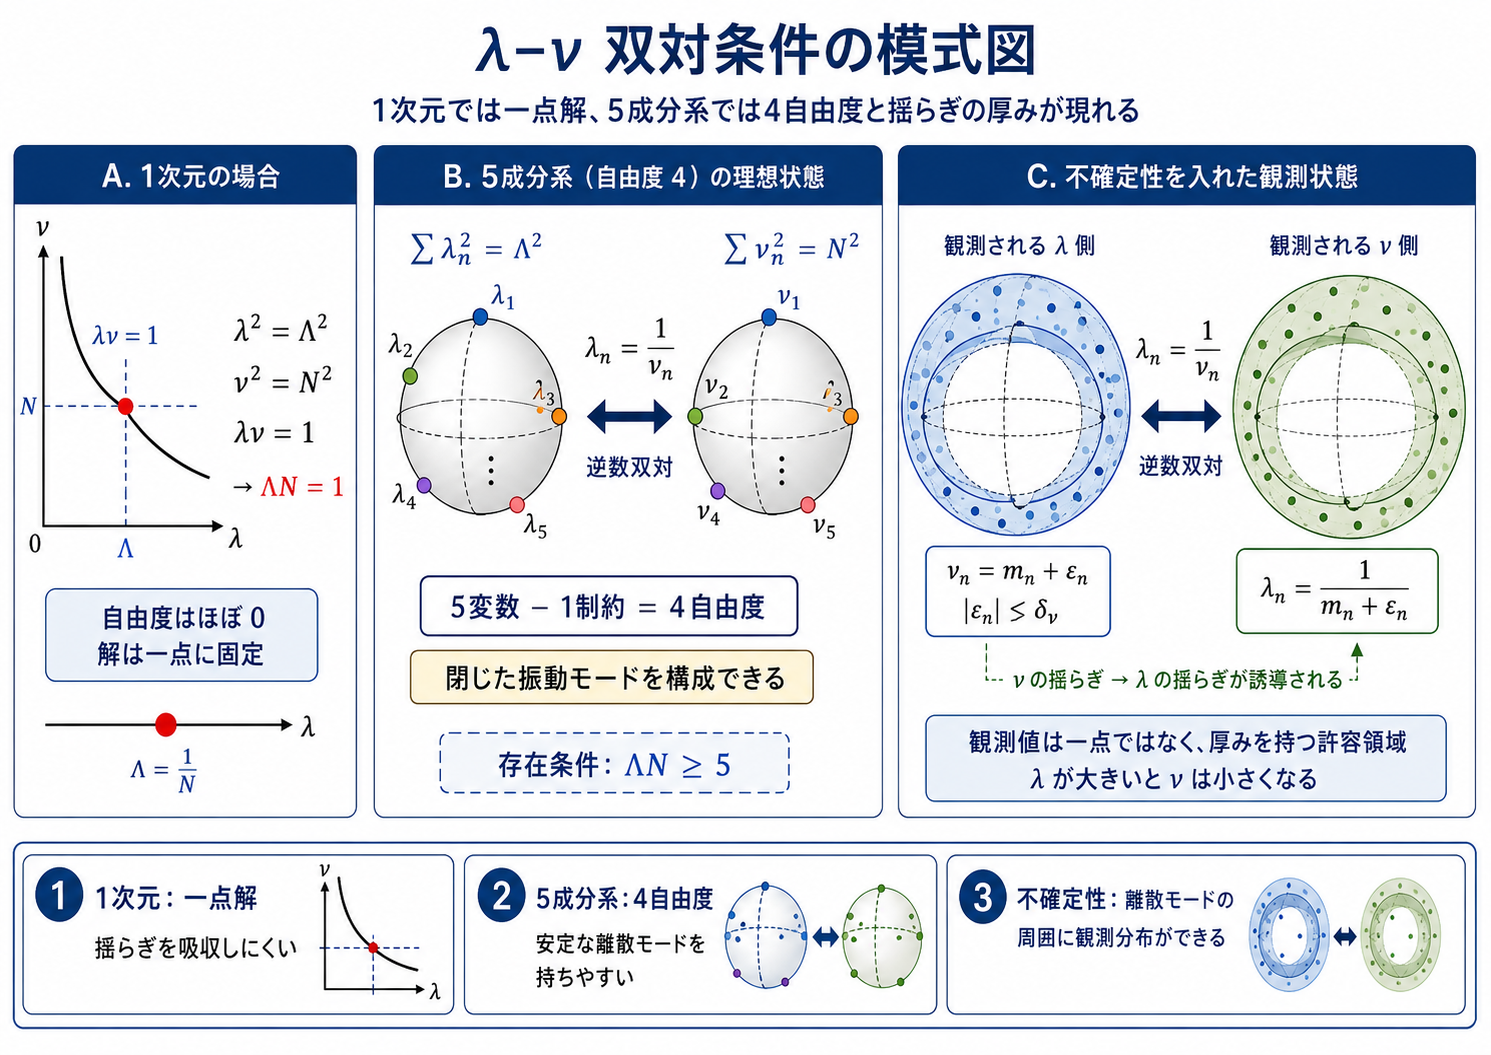
\includegraphics[keepaspectratio,alt={λ--ν 双対条件の模式図}]{./λ_ν_双対条件の模式図.png}}
\caption{λ--ν 双対条件の模式図}
\end{figure}

\textbf{図1.}
1次元では、\(\lambda^2=\Lambda^2\)、\(\nu^2=\mathcal{N}^2\)、\(\lambda\nu=1\)
の条件により解はほぼ一点に固定される。一方、5成分1制約の系では4自由度が残り、双対幾何を構成する余地が生じる。不確定性を導入すると、理想的な制約の周囲に厚みを持つ観測領域として表現できる。ただし、その厚みの大きさは本稿では導出しない。

\subsubsection{図2：λ--ν
双対の対数表現}\label{ux56f32ux3bbux3bd-ux53ccux5bfeux306eux5bfeux6570ux8868ux73fe}

\begin{figure}
\centering
\pandocbounded{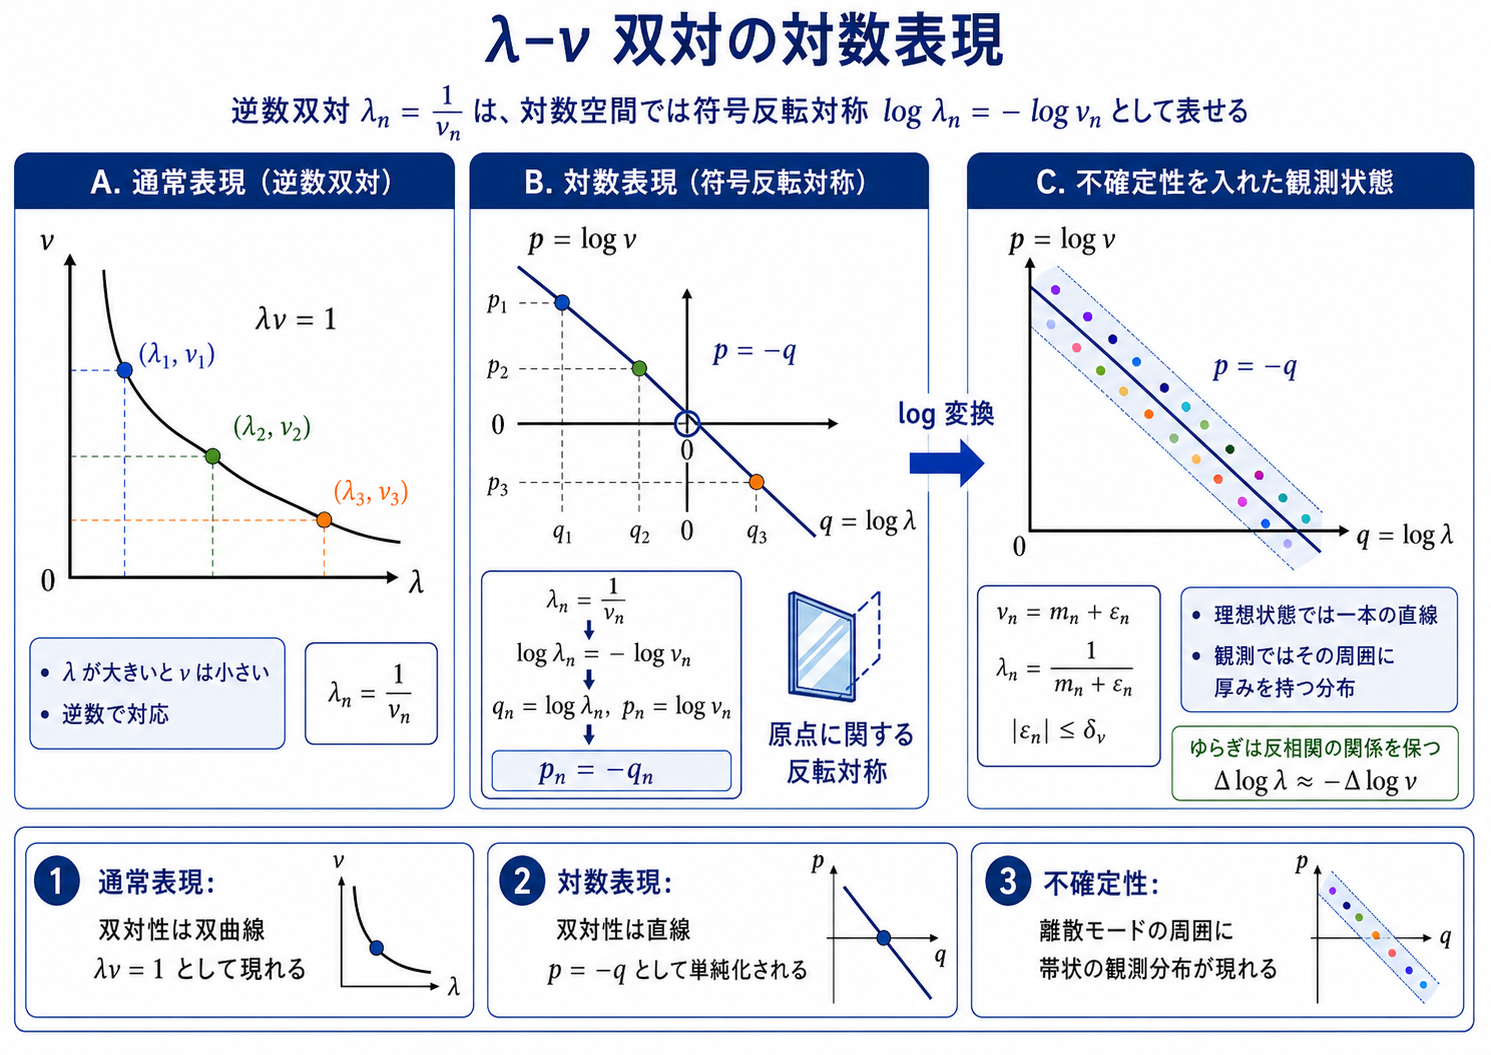
\includegraphics[keepaspectratio,alt={λ--ν 双対の対数表現}]{./λ_ν_双対の対数表現.png}}
\caption{λ--ν 双対の対数表現}
\end{figure}

\textbf{図2.} 通常表現では双曲線 \(\lambda\nu=1\)
として表される逆数双対は、対数変数 \(q=\log\lambda\)、\(p=\log\nu\)
を用いることで、直線 \(p=-q\)
として表される。不確定性を導入した観測状態では、理想直線の周囲に厚みを持つ帯状分布として表現しうる。ただし、本稿ではその厚みを決定しない。

\begin{center}\rule{0.5\linewidth}{0.5pt}\end{center}

\subsection{8.
実際の周波数空間・波長空間における4次元格子数え上げ}\label{ux5b9fux969bux306eux5468ux6ce2ux6570ux7a7aux9593ux6ce2ux9577ux7a7aux9593ux306bux304aux3051ux308b4ux6b21ux5143ux683cux5b50ux6570ux3048ux4e0aux3052}

ここまでの議論は、連続的な双対空間を主に扱ってきた。しかし、周波数空間または波長空間を実際に4次元格子として選ぶと、二乗和条件は自然に単位セルの数え上げ問題に変換できる。

\subsubsection{\texorpdfstring{8.1 \(\delta=0\)
の完全内接数え上げ}{8.1 \textbackslash delta=0 の完全内接数え上げ}}\label{delta0-ux306eux5b8cux5168ux5185ux63a5ux6570ux3048ux4e0aux3052}

4次元整数格子

\[
k=(k_1,k_2,k_3,k_4)\in\mathbb{Z}^4
\]

を考える。

一辺1の4次元単位セルを各格子点 \(k\)
に対応させる。単位セルの各方向の半幅は \(1/2\) である。

半径 \(R\)
の4次元超球体に、この単位セル全体が完全に内接するための条件は、

\[
\sum_{i=1}^{4}
\left(|k_i|+\frac12\right)^2
\le R^2
\]

である。

したがって、\(\delta=0\) における完全内接セル数を

\[
N_0(R)
=
\#\left\{
k\in\mathbb{Z}^4
\mid
\sum_{i=1}^{4}
\left(|k_i|+\frac12\right)^2
\le R^2
\right\}
\]

と定義する。

この定義は、周波数空間に4次元格子を選んだ場合にも、波長空間に4次元格子を選んだ場合にも、同じ形式で適用できる。ここで数えているのは、特定の物理量ではなく、二乗和制約を持つ4次元格子セルの幾何学的個数である。

整数半径について順に数えると、例えば

\[
N_0(1)=1,\qquad
N_0(2)=9,\qquad
N_0(3)=137
\]

を得る。

特に \(R=3\)
で得られる137は、物理定数との対応を仮定して導入されたものではない。4次元整数格子、単位セル、完全内接条件から得られる純粋な数え上げ結果である。

\subsubsection{8.2
不確定性を含む数え上げの形式}\label{ux4e0dux78baux5b9aux6027ux3092ux542bux3080ux6570ux3048ux4e0aux3052ux306eux5f62ux5f0f}

不確定性を含まない完全内接数え上げでは、各セルは条件を満たせば1、満たさなければ0として数えられる。これは指示関数

\[
\mathbf{1}[x\ge 0]
\]

による数え上げである。

ここで、

\[
D_R(k)
=
R^2-
\sum_{i=1}^{4}
\left(|k_i|+\frac12\right)^2
\]

を定義する。

\[
D_R(k)\ge0
\]

なら、その単位セルは半径 \(R\) の超球体に完全に内接する。

不確定性を含む場合、指示関数を、境界近傍に厚みを持つ重み関数

\[
W_\delta(x)
\]

に置き換える。

このとき、有効セル数を

\[
N_\delta(R)
=
\sum_{k\in\mathbb{Z}^4}
W_\delta\!\left(
D_R(k)
\right)
\]

と定義する。

重み関数は、少なくとも次の性質を満たすものとする。

\[
0\le W_\delta(x)\le1,
\]

\[
\lim_{\delta\to0}
W_\delta(x)
=
\mathbf{1}[x\ge0].
\]

したがって、

\[
\lim_{\delta\to0}N_\delta(R)=N_0(R)
\]

である。

この定式化により、完全内接数え上げは、不確定性を含む重み付き数え上げの
\(\delta=0\) 極限として表される。

ただし、本稿では \(W_\delta\) の具体的な形、\(\delta\) の値、または
\(\delta\) がどの幾何量に依存するかを導出しない。したがって、本稿では
\(N_\delta(R)\) の具体的な数値評価は行わない。

\subsubsection{8.3
双対数え上げの注意}\label{ux53ccux5bfeux6570ux3048ux4e0aux3052ux306eux6ce8ux610f}

周波数空間に4次元格子を置く場合、二乗和条件

\[
\sum_{i=1}^{4} \nu_i^2\le \mathcal{N}^2
\]

に対応する単位セル数え上げを行うことができる。

一方、波長空間に4次元格子を置く場合は、

\[
\sum_{i=1}^{4} \lambda_i^2\le \Lambda^2
\]

に対応する単位セル数え上げを行うことができる。

両者は形式的には同じ数え上げ問題である。しかし、波長空間と周波数空間は

\[
\lambda_i\nu_i=1
\]

によって双対的に結ばれるため、両者を同時に格子化したときには、各空間の格子構造が単純に一致するとは限らない。

したがって、本稿では次の二つを区別する。

\begin{enumerate}
\def\labelenumi{\arabic{enumi}.}
\tightlist
\item
  周波数空間または波長空間を単独で4次元格子として選んだときの数え上げ。\\
\item
  両者を逆数双対条件で同時に結びつけたときの整合条件。
\end{enumerate}

本稿では、まず1の単独空間での数え上げを定義するに留める。2の双対整合条件を含む数え上げは、後続研究の課題とする。

\begin{center}\rule{0.5\linewidth}{0.5pt}\end{center}

\subsection{9.
関連研究と位置づけ}\label{ux95a2ux9023ux7814ux7a76ux3068ux4f4dux7f6eux3065ux3051}

本稿は、既存の物理理論を修正するものではなく、波長空間と周波数空間の間に逆数双対条件を置いたときに現れる幾何学的構造を観察するモデルである。したがって、以下の関連研究は、本稿の主張の物理的根拠ではなく、数理的背景として参照する。

第一に、信号解析において時間領域と周波数領域を相補的に扱う考え方は、Gabor
の時間--周波数解析に代表される古典的背景を持つ。Gabor
は通信信号の解析において、時間と周波数を対称的に扱う方法を提示した
{[}1{]}。本稿は時間軸を物理的に導入するものではないが、双対空間を並置して観察するという形式的動機を共有する。

第二に、周波数領域や情報表現の抽象化という点では、Shannon
の通信理論が古典的背景を与える
{[}2{]}。ただし、本稿では情報量や通信路容量を扱わない。

第三に、本稿末尾の4次元格子セル数え上げは、凸体内の格子点または格子セルを扱う数の幾何（geometry
of numbers）の文脈に属する。特に、Minkowski
以降の数の幾何は、凸体、格子、体積、数え上げの関係を体系的に扱ってきた
{[}3{]}。

第四に、4次元格子上の二乗和条件は、4つの平方和の表現数と形式的に近い。ただし、本稿で扱うのは正の奇数平方和に基づく不等式条件であり、Jacobi
の四平方定理を直接適用するものではない {[}4{]}。

\begin{center}\rule{0.5\linewidth}{0.5pt}\end{center}

\subsection{10.
限界と今後の課題}\label{ux9650ux754cux3068ux4ecaux5f8cux306eux8ab2ux984c}

本稿には明確な限界がある。

第一に、本稿は物理理論を完成させるものではない。波長、周波数、ノルム保存、不確定性という語を用いているが、それらを既存物理量と直接同一視していない。

第二に、\(\lambda_n\) および \(\nu_n\)
の物理次元、単位系、観測可能量との対応は未定義である。

第三に、4自由度構造が唯一であることは示していない。本稿で示したのは、1次元では自由度が不足し、5成分1制約では4自由度が自然に現れるという観察である。

第四に、不確定性幅 \(\delta\)
の値や分布を本稿では決定しない。特に、重み関数 \(W_\delta\)
の形、\(\delta\)
が境界距離、殻番号、対数空間での双対整合誤差などのどの量に依存するかは、本稿のスコープ外である。

第五に、周波数空間と波長空間を同時に格子化し、さらに逆数双対条件を満たす整合数え上げをどのように行うかは、今後の課題である。

\begin{center}\rule{0.5\linewidth}{0.5pt}\end{center}

\subsection{11. 結論}\label{ux7d50ux8ad6}

本稿では、波長成分 \(\lambda_n\) と周波数成分 \(\nu_n\)
の間に逆数双対条件

\[
\lambda_n=\frac{1}{\nu_n}
\]

を置き、さらに波長空間と周波数空間にそれぞれ二乗和一定条件を課したときに現れる幾何学的構造を観察した。

1次元の場合、解はほぼ一点に固定され、成分間の再配分余地をほとんど持たない。一方、5成分1制約の系では4自由度が残る。

また、対数変数を導入すると、逆数双対は

\[
p_n=-q_n
\]

という符号反転対称として表される。

最後に、実際の周波数空間または波長空間を4次元格子として選んだ場合、二乗和条件は単位セル数え上げ問題として定式化できることを示した。不確定性を含まない
\(\delta=0\) の場合には、完全内接セル数 \(N_0(R)\)
が得られる。さらに、不確定性を含む場合には、指示関数を重み関数
\(W_\delta\) に置き換えた有効セル数 \(N_\delta(R)\) として定式化できる。

ただし、本稿では \(\delta\) の値や \(W_\delta\)
の具体形を導出しない。これらは本稿のスコープ外であり、後続研究の課題である。

\begin{center}\rule{0.5\linewidth}{0.5pt}\end{center}

\subsection{\texorpdfstring{付録A：一般 \(d\)
成分系の存在条件}{付録A：一般 d 成分系の存在条件}}\label{ux4ed8ux9332aux4e00ux822c-d-ux6210ux5206ux7cfbux306eux5b58ux5728ux6761ux4ef6}

一般の \(d\) 成分系において、

\[
\sum_{n=1}^{d} \lambda_n^2=\Lambda^2,\qquad
\sum_{n=1}^{d} \nu_n^2=\mathcal{N}^2,\qquad
\lambda_n\nu_n=1
\]

を課す。

\[
a_n=\lambda_n^2>0
\]

と置くと、

\[
\sum_{n=1}^{d} a_n=\Lambda^2,\qquad
\sum_{n=1}^{d} \frac{1}{a_n}=\mathcal{N}^2
\]

である。

Cauchy--Schwarz 型の不等式より、

\[
\left(\sum_{n=1}^{d} a_n\right)
\left(\sum_{n=1}^{d} \frac{1}{a_n}\right)\ge d^2
\]

である。

したがって、

\[
\Lambda\mathcal{N}\ge d
\]

が必要条件となる。

\begin{center}\rule{0.5\linewidth}{0.5pt}\end{center}

\subsection{参考文献}\label{ux53c2ux8003ux6587ux732e}

\begin{enumerate}
\def\labelenumi{\arabic{enumi}.}
\item
  Gabor, D. (1946). Theory of communication. \emph{Journal of the
  Institution of Electrical Engineers - Part III: Radio and
  Communication Engineering}, 93(26), 429--457.
\item
  Shannon, C. E. (1948). A mathematical theory of communication.
  \emph{Bell System Technical Journal}, 27(3), 379--423.
\item
  Aliev, I., \& Henk, M. (2023). Minkowski's successive minima in convex
  and discrete geometry. \emph{Communications in Mathematics}, 31(2),
  35--59.
\item
  Hirschhorn, M. D. (1987). A simple proof of Jacobi's four-square
  theorem. \emph{Proceedings of the American Mathematical Society},
  101(3), 436--438.
\end{enumerate}

\begin{center}\rule{0.5\linewidth}{0.5pt}\end{center}

\subsection{図ファイル}\label{ux56f3ux30d5ux30a1ux30a4ux30eb}

\begin{itemize}
\tightlist
\item
  図1：\texttt{λ\_ν\_双対条件の模式図.png}
\item
  図2：\texttt{λ\_ν\_双対の対数表現.png}
\end{itemize}

\end{document}
